\section{Background Estimation}
\label{sec:llvv_background}

In the measurement of the $\text{ZZ} \to \ell^+\ell^-\nu\bar{\nu}$ cross-section, several background processes contribute. These can be categorized as follows:

\begin{itemize}

    % --- FIRST TOP-LEVEL ITEM ---
    \item \textbf{Irreducible Backgrounds}
    \begin{itemize}
        \item \textbf{Diboson processes:}
        \begin{itemize}
            \item $\text{WW} \to \ell\nu\ell\nu$: The two neutrinos contribute to the $E_{\text{T}}^{\text{miss}}$ signature, faking the $\text{ZZ} \to \ell\ell\nu\nu$ process.
            \item $\text{WZ} \to \ell\nu\ell\ell$: If one lepton from the $\text{Z}$ is missing in detection, this process could fake the signal.
            \item $\text{ZZ} \to \ell\ell\ell\ell$: If two leptons escape detection, this process contributes as a background.
        \end{itemize}
    \end{itemize}

    % --- SECOND TOP-LEVEL ITEM ---
    \item \textbf{Reducible Backgrounds}
    \begin{itemize}
        \item \textbf{Top-quark backgrounds:}
        \begin{itemize}
            \item $t\bar{t}$: If $b$-jets in the $t\bar{t}$ final states are not tagged properly, it may fake the signal.
            \item Single top ($\text{W}t$): It can contribute similarly to the $t\bar{t}$ background.
        \end{itemize}
        \item \textbf{Drell--Yan + jets} ($\text{Z} \to \ell\ell$ + jets): Jet energy mismeasurement can lead to artificial $E_{\text{T}}^{\text{miss}}$.
        \item \textbf{$\text{W}$ + jets}: A single $\text{W}$ boson decaying leptonically with jets can mimic the signal region due to misidentification of a jet as a faked lepton.
    \end{itemize}

\end{itemize}

To achieve precise cross-section measurements, these backgrounds must be carefully estimated using the background control regions. Considering the final states of the backgrounds, they can be categorized into the following Control Regions (CRs):

\begin{itemize}
    \item \textbf{Non-Resonant Backgrounds} (from $t\bar{t}, \text{W}t, \text{WW}, \tau\tau$):\\
    These processes decay via two $\text{W}$ bosons (or $\tau$ leptons) rather than a $\text{Z}$ boson, resulting in uncorrelated lepton flavors. They are further categorized by $b$-jet multiplicity to separate Top processes from $\text{WW}$ processes:
    \begin{itemize}
        \item \textbf{0 $b$-jet Category ($\text{WW}$ Enriched):}
        \begin{itemize}
            \item $\text{WW} \to \ell\nu\ell\nu$: The dominant contribution in the 0 $b$-tag phase space. The neutrinos create genuine $E_{\text{T}}^{\text{miss}}$.
            \item $t\bar{t}$ / Single Top ($\text{W}t$): Top events contribute to this category only if the $b$-jets fail to be identified (tagging inefficiency) or fall outside detector acceptance.
        \end{itemize}
        \item \textbf{$\ge 1$ $b$-jet Category (Top Enriched):}
        \begin{itemize}
             \item $t\bar{t} \to \text{W}b\text{W}b$ and $\text{W}t$: The dominant contribution when at least one $b$-jet is identified. These events contain real $E_{\text{T}}^{\text{miss}}$ from the $\text{W}$ decays.
        \end{itemize}
    \end{itemize}

    \item \textbf{3-Lepton Backgrounds ($\text{WZ}$)}
    \begin{itemize}
        \item $\text{WZ} \to \ell\nu\ell\ell$: This is an irreducible background if one of the three leptons is lost (fails reconstruction) or falls outside the detector acceptance, mimicking the $2\ell + E_{\text{T}}^{\text{miss}}$ signature.
    \end{itemize}
    
    \item \textbf{$\text{Z}$+Jets Backgrounds (Instrumental $E_{\text{T}}^{\text{miss}}$)}
    \begin{itemize}
        \item \textbf{Drell--Yan + jets} ($\text{Z}/\gamma^* \to \ell\ell$ + jets): The dominant reducible background. It contains real leptons from the $\text{Z}$ boson, but the $E_{\text{T}}^{\text{miss}}$ is artificial (``fake''), caused by jet energy mismeasurement or pile-up interactions.
    \end{itemize}
   
    \item \textbf{Fake Lepton / Instrumental Backgrounds}
    \begin{itemize}
        \item \textbf{$\text{W}$ + jets}: A process with one real lepton from a $\text{W}$ boson and a jet misidentified as a second lepton (fake lepton), creating a fake $2\ell$ signature.
        \item \textbf{Fake $E_{\text{T}}^{\text{miss}}$}: Detector anomalies, cosmic-ray muons, or beam halo effects that produce large artificial missing energy.
    \end{itemize}
\end{itemize}

To accurately estimate background contributions, dedicated control regions (CRs) are defined, each enriched in a specific background process. A simultaneous fit is performed across all CRs and the signal region to constrain both the yields and shapes of these backgrounds consistently. The fit uses event distributions as inputs and derives scale factors that adjust the MC predictions to match the data in the CRs. These scaled MC predictions are then extrapolated to the signal region to provide reliable background estimates, forming the basis for the cross-section measurement.

The following sections describe the estimation strategy for each control region in detail.

\subsection{Non-Resonant Background in $e^\pm\mu^\mp$ CR (With/Without $b$-Jet)}
\label{sec:bkg_emuCR}

Considering the high percentage of the non-resonant backgrounds, it would be better if the control regions are well defined to control the backgrounds from MC estimations. Therefore, 2 Control Regions are defined to further estimate the yields from those processes. 

One is the non-resonant background, which requires different-flavour opposite-sign (DFOS) leptons ($e^\pm\mu^\mp$) in the final state. For example, in the $\text{WW} \to \ell\nu\ell\nu$ process, the observable final state could be either same-flavour opposite-sign (SFOS) leptons, which fakes the true signals, or different-flavour opposite-sign (DFOS) leptons. Considering that there is an equal chance for the $\text{W}$ boson to decay to an electron or muon, the yield ratio between SFOS and DFOS final states would be 1:1 (considering both $ee \ \text{and} \ \mu\mu$ SFOS). Since the DFOS events are well separated from the SFOS, this would be a good approach to estimate the background yields in the Signal Region (SR) using the CR events. 

However, since the final state from top quark pair or single top decay contains 1 or 2 $b$-jets, the observed final state could contain 1 or more $b$-jets. Therefore, define a CR with a 1 $b$-jet to further estimate the yield from top backgrounds. The non-resonant with zero $b$-jet CR definition is the same as the common non-resonant CR, except for the $b$-jet tagging requirement. For the VBS-like $\text{ZZ}jj$ analysis, the non-resonant CR contains both $\text{WW}$ and top background events. 

Since this aims to estimate yields in the SR, the non-resonant background definition is the same as in the SR, except that it requires DFOS events. The detailed definitions of non-resonant with/without 1 $b$-jet are shown in Table~\ref{tab:em_definition}. The pre-fit distributions of $\Delta\phi(\vec{E}_{\text{T}}^{\text{miss}}, \text{Z})$ in the CRs for both data and MC prediction are shown in Figure~\ref{fig:em-CR-prefit}. The purity of the non-resonant background events exceeds 99\% in the CRs.

\begin{table}[!htbp]
\centering
\renewcommand{\arraystretch}{1.2}
\begin{tabular}{|>{\centering\arraybackslash}p{4.5cm}|>{\centering\arraybackslash}p{4.5cm}|}
\hline
\multicolumn{2}{|c|}{Inclusive $\text{ZZ}$ phase space: $t\bar{t}$ / $\text{WW}$ $e\mu$ Control Region cuts} \\
\hline
\multicolumn{2}{|c|}{$80 < m_{\ell\ell} < 100~\text{GeV}$} \\
\hline\multicolumn{2}{|c|}{$E_{\text{T}}^{\text{miss}} > 70~\text{GeV}$} \\
\hline\multicolumn{2}{|c|}{$\Delta R_{\ell\ell} < 2$} \\
\hline\multicolumn{2}{|c|}{$\Delta\phi(\vec{E}_{\text{T}}^{\text{miss}}, \vec{p}_{\text{T}}^{\,e\mu}) > 2.2$} \\
\hline\multicolumn{2}{|c|}{$E_{\text{T}}^{\text{miss}}/H_{\text{T}} > 0.3$} \\
\hline
$b$-jet veto ($\text{WW}$) & $n_{b\text{-jet}} > 0$ (top) \\
\hline
\end{tabular}
\caption{Definition of $t\bar{t}$ / $\text{WW}$ $e\mu$ Control Region in inclusive $\text{ZZ}$ measurement phase-space.}
\label{tab:em_definition}
\end{table}

\begin{figure}[!htbp]
    \centering
    \subfloat[]{
    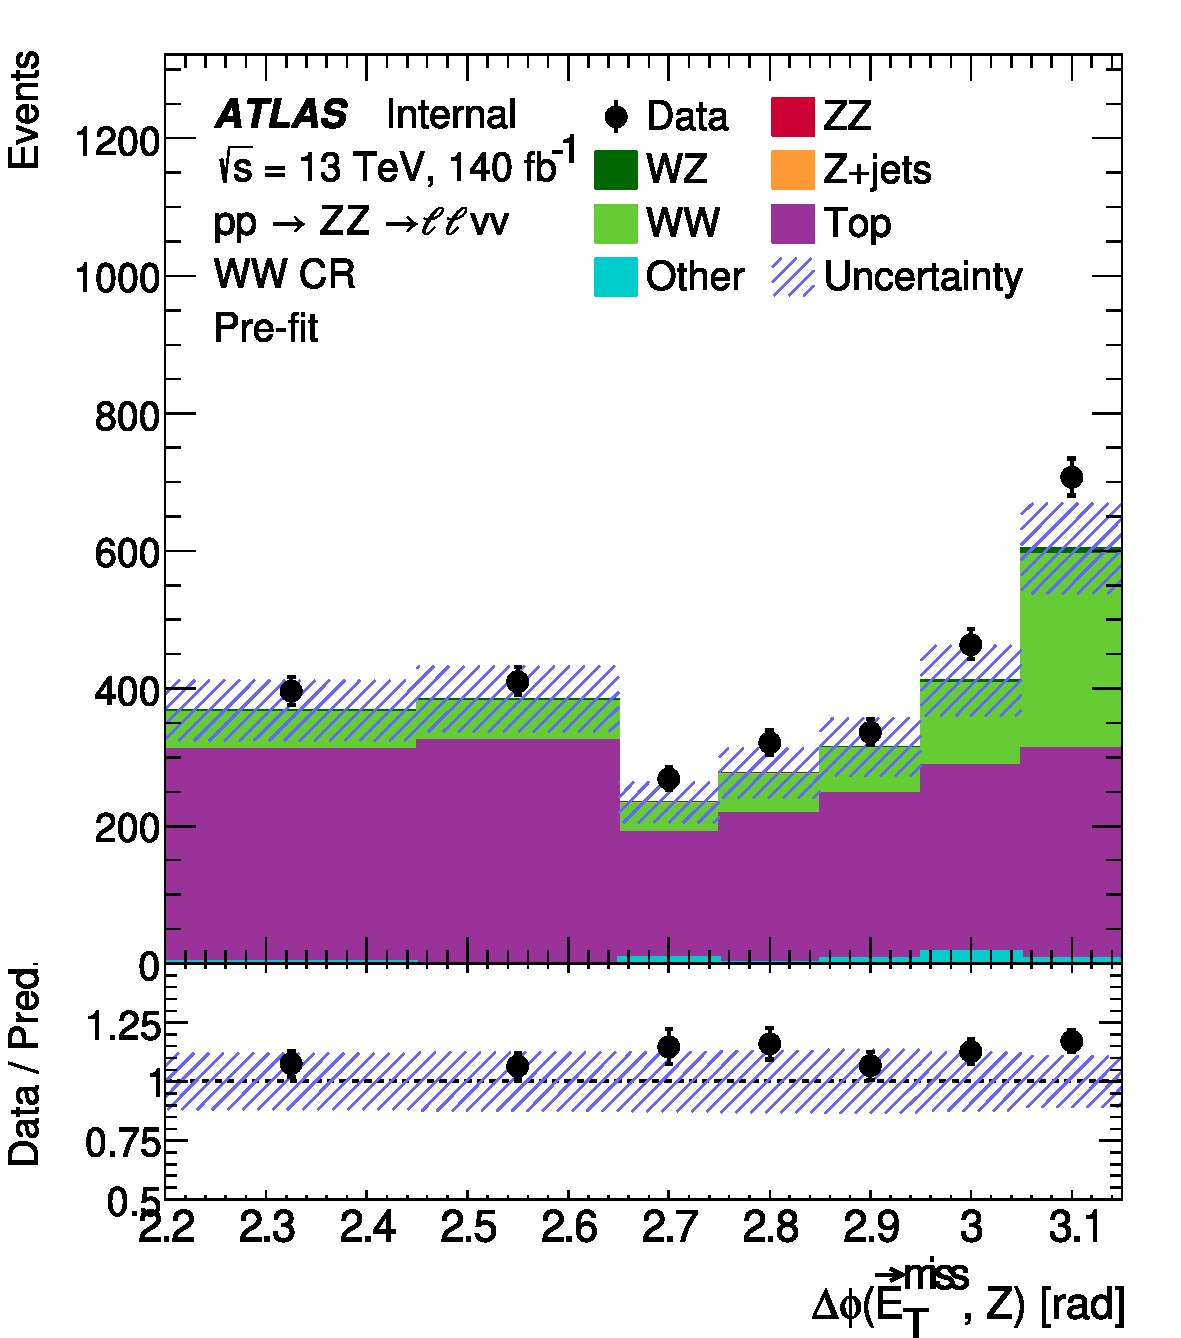
\includegraphics[width=0.32\linewidth]{figures/ch5-llvv/kin-distribution/EMU_A-ZZ.pdf}}
    \subfloat[]{    
    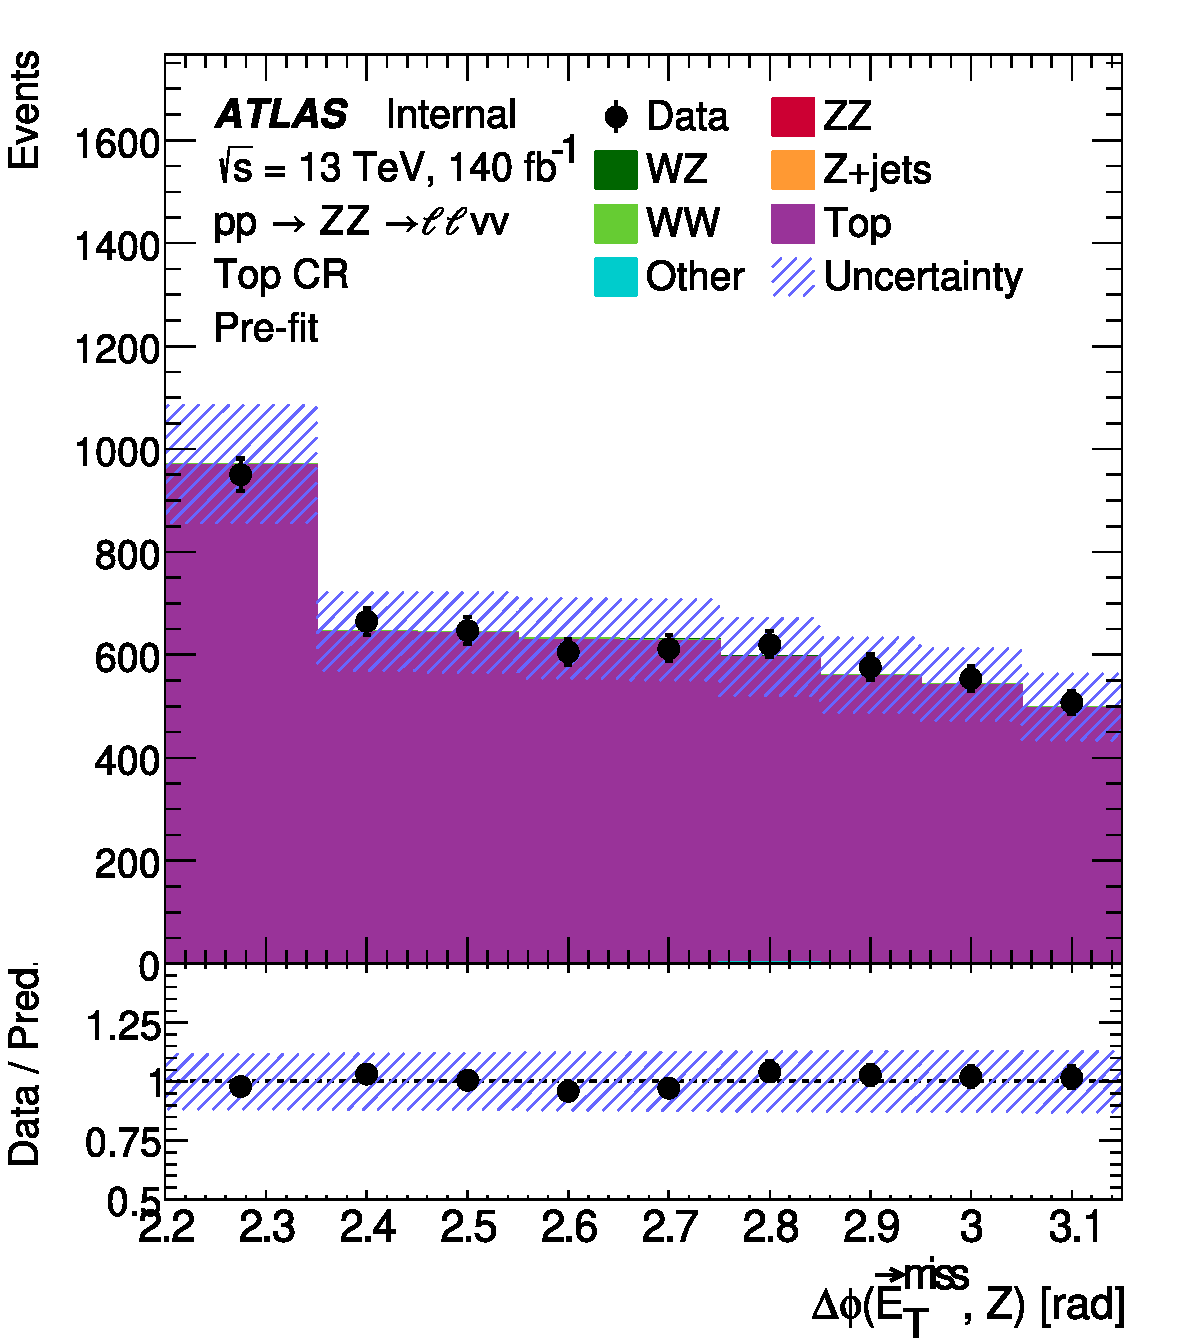
\includegraphics[width=0.32\linewidth]{figures/ch5-llvv/kin-distribution/EMU_B-ZZ.pdf}}
   \subfloat[]{    
    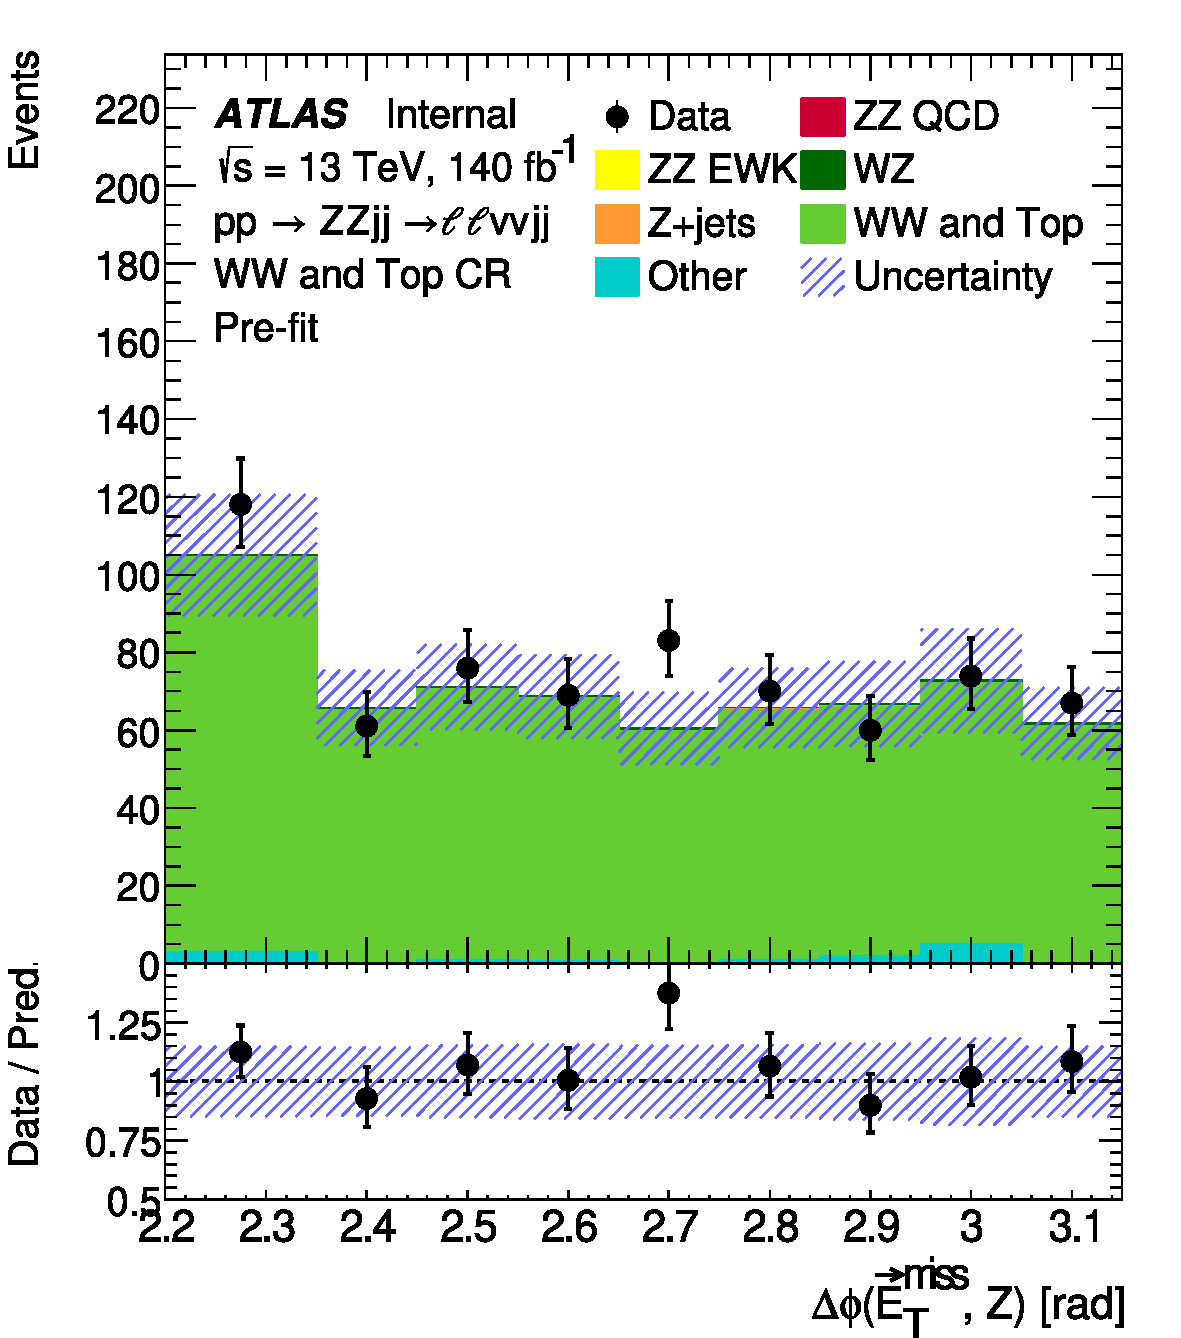
\includegraphics[width=0.32\linewidth]{figures/ch5-llvv/kin-distribution/EMU-ZZjj.pdf}}
    \caption{Data and MC (pre-fit) comparison of the $\Delta\phi(\vec{E}_{\text{T}}^{\text{miss}}, \text{Z})$ in the $e\mu$ CRs for inclusive $\text{ZZ}$ analysis: (a) $\text{WW}$ CR (no $b$-jet), (b) Top CR (with $b$-jets), and (c) for VBS-like $\text{ZZ}jj$ analysis.}
    \label{fig:em-CR-prefit}
\end{figure}

\subsection{3-Lepton Control Region (3$\ell$ CR)}
\label{sec:bkg_3lCR}

The $\text{WZ} \to \ell\nu\ell\ell$ process constitutes a major irreducible background for the $\text{ZZ} \to \ell\ell\nu\nu$ analysis. This process mimics the signal topology if one of the three leptons fails to be reconstructed or falls outside the detector acceptance, resulting in apparent missing transverse energy. To constrain the normalization and modeling of the $\text{WZ}$ background, an inclusive 3-lepton Control Region (3$\ell$ CR) is defined.

\subsubsection{Definition and Event Selection}

The selection criteria for the 3$\ell$ CR are summarized in Table~\ref{table:3lCR_definition_sim}. The primary requirement distinguishing this region from the Signal Region (SR) is the lepton multiplicity; we require the presence of more than two leptons ($n_{\text{leptons}} > 2$). This condition ensures strictly orthogonal phase spaces between the control and signal regions, preventing any event overlap.
\begin{table}[!htbp]
\centering
\begin{tabular}{|l|c|}
\hline
\textbf{Variable} & \textbf{Cut Value} \\ 
\hline 
$n_{\text{leptons}}$ & $> 2$ \\
\hline 
$m_{\ell\ell}$ & $80 < m_{\ell\ell} < 100~\text{GeV}$ \\
\hline 
$E_{\text{T}}^{\text{miss}}$ & $> 70~\text{GeV}$ \\
\hline 
$\Delta R_{\ell\ell}$ & $< 2$ \\ 
\hline 
$\Delta \varphi(E_{\text{T}}^{\text{miss}}, \text{Z})$ & $> 2.2 $ \\
\hline 
$E_{\text{T}}^{\text{miss}} / H_{\text{T}}$ & $> 0.3$ \\
\hline 
Heavy Flavor & $b$-jet veto \\
\hline 
$m_{\text{T, W}}$ & $> 30~\text{GeV}$ \\ 
\hline
\end{tabular}
\caption{Definition of the inclusive 3-lepton Control Region (3$\ell$ CR). The kinematic selections mimic the Signal Region to ensure phase-space compatibility, while the lepton multiplicity ensures orthogonality.}
\label{table:3lCR_definition_sim}
\end{table}

Apart from the lepton multiplicity, the kinematic cuts are chosen to closely mirror those of the Signal Region. This strategy ensures that the control region probes a phase space with similar kinematic characteristics to the signal region, thereby minimizing systematic uncertainties associated with extrapolating the normalization factors (scaling factors) from the CR to the SR. However, certain cuts are kept slightly looser than in the SR to retain higher statistics, reducing the statistical uncertainty on the derived scaling factors.
\begin{figure}[!htbp]
    \centering
    \subfloat[]{
    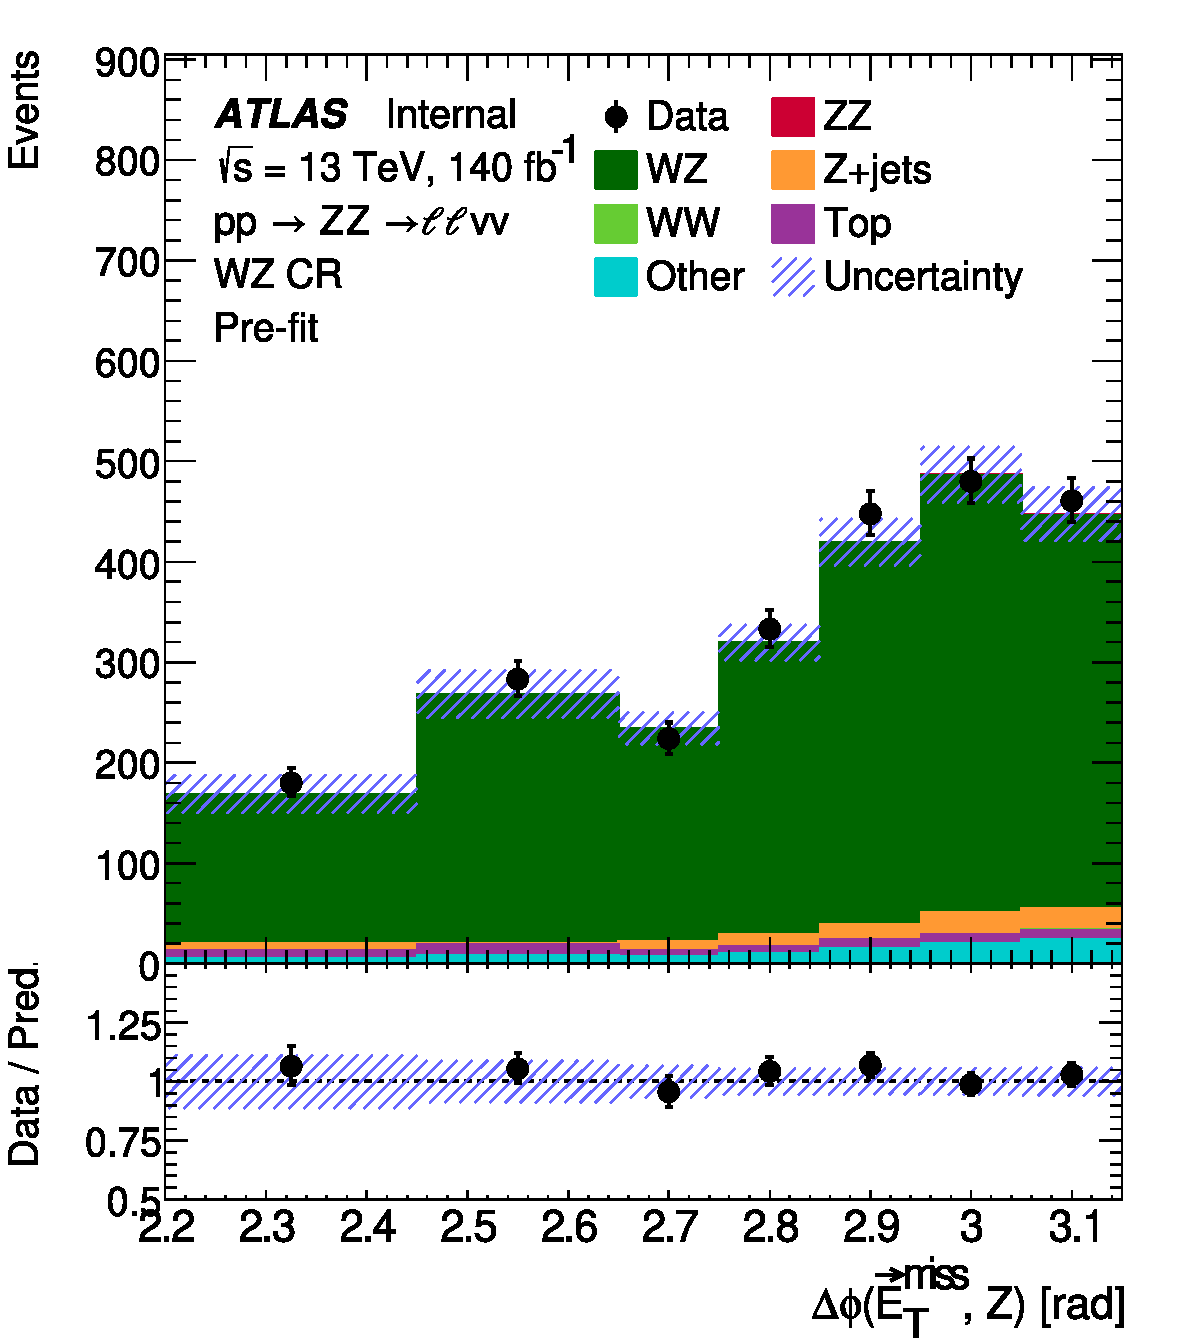
\includegraphics[width=0.45\linewidth]{figures/ch5-llvv/kin-distribution/WZ-ZZ.pdf}}
    \subfloat[]{
    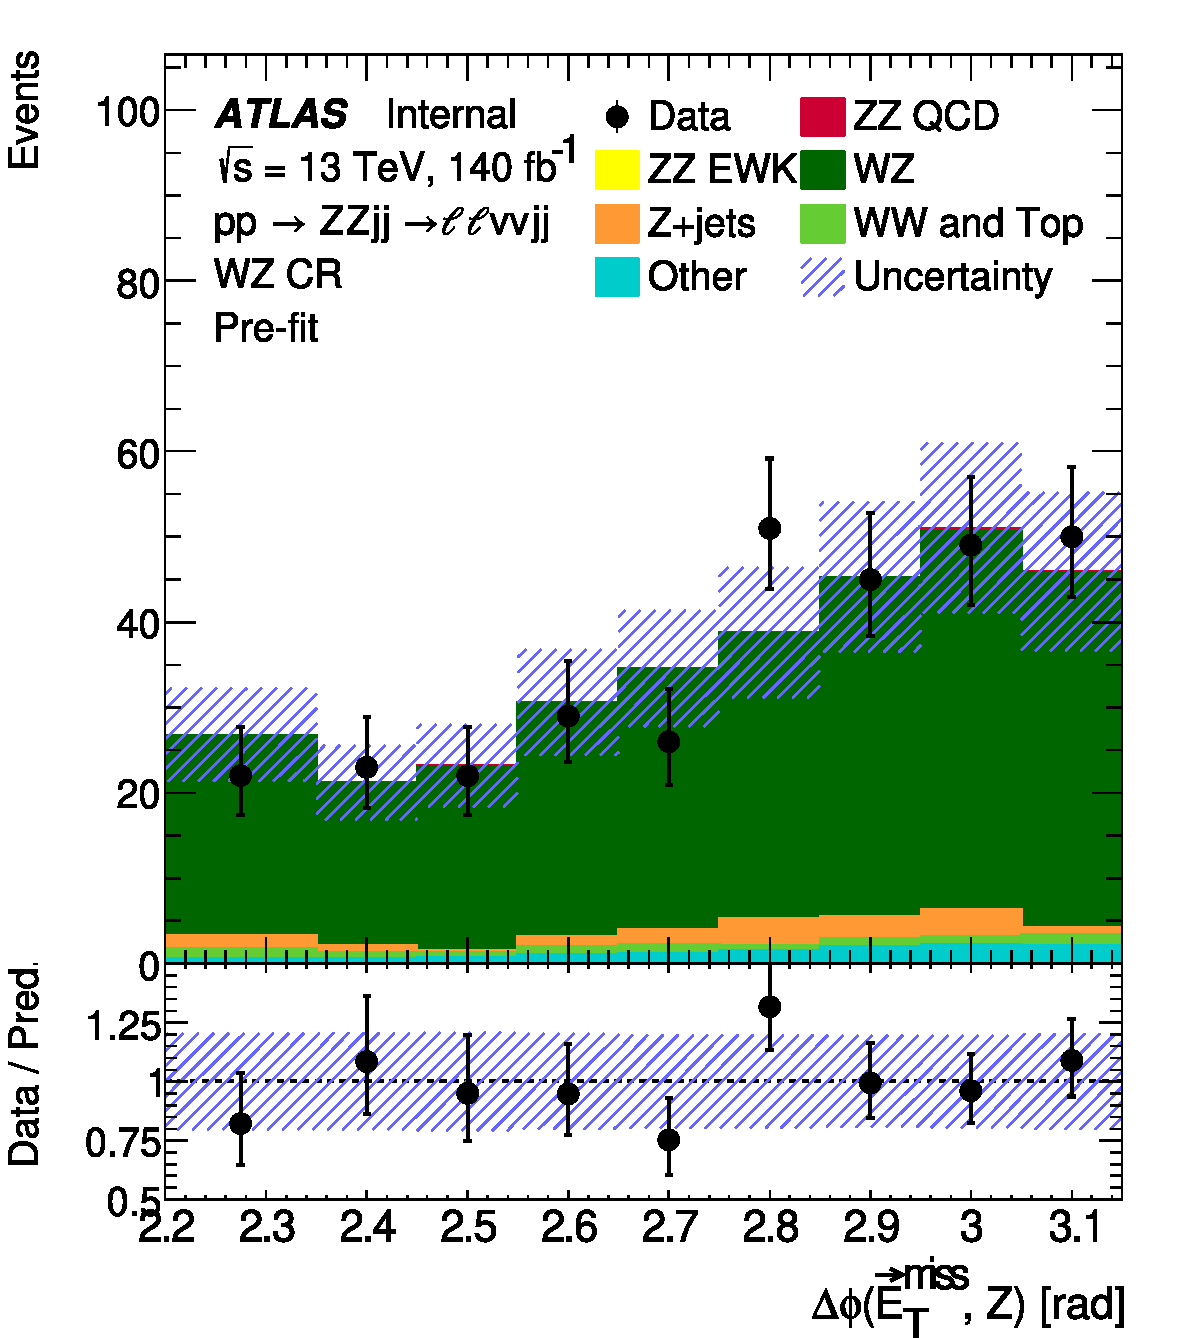
\includegraphics[width=0.45\linewidth]{figures/ch5-llvv/kin-distribution/WZ-ZZjj.pdf}}
    \caption{Data and MC (pre-fit) comparison of the $\Delta\phi(\vec{E}_{\text{T}}^{\text{miss}}, \text{Z})$ in the $\text{WZ}$ 3$\ell$ CR: (a) for the inclusive $\text{ZZ}$ analysis, and (b) for the VBS-like $\text{ZZ}jj$ analysis. }
    \label{fig:3l-CR-prefit}
\end{figure}

Specifically, the selection requires an opposite-sign same-flavour (OSSF) lepton pair consistent with the $\text{Z}$ boson mass ($80 < m_{e\mu} < 100~\text{GeV}$). To select a topology consistent with the high-$p_{\text{T}}$ $\text{Z}$ boson signal, a large missing transverse energy cut ($E_{\text{T}}^{\text{miss}} > 70~\text{GeV}$) and a boost requirement on the leptons ($\Delta R_{\ell\ell} < 2$) are applied.

Furthermore, a transverse mass cut is applied to the third lepton and the $E_{\text{T}}^{\text{miss}}$, denoted as $m_{\text{T, W}} > 30~\text{GeV}$. This cut is introduced specifically to suppress the contribution from $\text{Z}$+jets events where a jet is misidentified as a lepton. By requiring a non-zero $m_{\text{T, W}}$, we reduce the contamination from non-prompt leptons, ensuring high purity of the $\text{WZ}$ process.

The pre-fit distributions of $\Delta\phi(\vec{E}_{\text{T}}^{\text{miss}}, \text{Z})$ for both $\text{ZZ}$ and $\text{ZZ}jj$ analyses in the $\text{WZ}$ 3$\ell$ CR for both data and MC prediction are shown in Figure~\ref{fig:3l-CR-prefit}. The purity of the $\text{WZ}$ background events exceeds 90\% in the CR.

\subsubsection{Composition and Yields}

The pre-fit event yields in the inclusive 3$\ell$ Control Region are presented in Table~\ref{table:3lCR_unscaled}. The region is dominated by the $\text{WZ}$ process, which accounts for approximately 90\% of the total background expectation, confirming the high purity of this control region.
\begin{table}[htbp]
\centering
\resizebox{\textwidth}{!}{%
\begin{tabular}{|l|c|c|c|c|c|}
\hline
\textbf{Process} & \textbf{All Channels} & \textbf{$\mu\mu\mu$} & \textbf{$\mu\mu e$} & \textbf{$\mu ee$} & \textbf{$eee$} \\ \hline
\textbf{Data} & \textbf{2409.0 $\pm$ 49.08} & 639.0 $\pm$ 25.28 & 607.0 $\pm$ 24.64 & 553.0 $\pm$ 23.52 & 610.0 $\pm$ 24.7 \\ \hline
\hline
EWK & 0.1 $\pm$ 0.01 & 0.01 $\pm$ 0.0 & 0.05 $\pm$ 0.01 & 0.04 $\pm$ 0.01 & 0.01 $\pm$ 0.0 \\ \hline
QCD & 2.4 $\pm$ 0.6 & 0.1 $\pm$ 0.13 & 1.47 $\pm$ 0.47 & 0.84 $\pm$ 0.31 & -0.01 $\pm$ 0.17 \\ \hline
\textbf{WZ} & \textbf{2106.3 $\pm$ 11.18} & 582.12 $\pm$ 5.83 & 536.64 $\pm$ 5.71 & 467.68 $\pm$ 5.55 & 519.85 $\pm$ 5.26 \\ \hline
$\text{Z}$+jets & 86.57 $\pm$ 11.0 & 20.56 $\pm$ 5.88 & 20.38 $\pm$ 5.77 & 28.37 $\pm$ 5.1 & 17.25 $\pm$ 5.21 \\ \hline
top, $t\bar{t}\text{V}$, $\text{W}t$ & 57.42 $\pm$ 1.83 & 9.19 $\pm$ 0.68 & 16.2 $\pm$ 0.97 & 18.76 $\pm$ 1.0 & 13.27 $\pm$ 0.97 \\ \hline
$\text{WW}$ & 0.65 $\pm$ 0.14 & 0.03 $\pm$ 0.03 & 0.21 $\pm$ 0.08 & 0.22 $\pm$ 0.08 & 0.2 $\pm$ 0.08 \\ \hline
Rare ($4\ell$, $\text{VVV}$, etc.) & 90.79 $\pm$ 1.35 & 31.86 $\pm$ 1.12 & 15.62 $\pm$ 0.35 & 14.73 $\pm$ 0.35 & 28.58 $\pm$ 0.58 \\ \hline
$\text{ZZ}$ & 2.5 $\pm$ 0.6 & 0.11 $\pm$ 0.0 & 1.52 $\pm$ 0.01 & 0.88 $\pm$ 0.01 & -0.01 $\pm$ 0.0 \\ \hline
\hline
\textbf{Total Bkg} & \textbf{2341.73 $\pm$ 15.85} & 643.85 $\pm$ 8.38 & 590.53 $\pm$ 8.2 & 530.61 $\pm$ 7.62 & 579.14 $\pm$ 7.49 \\ \hline
\hline
Data/MC & 1.03 $\pm$ 0.02 & 0.99 $\pm$ 0.04 & 1.03 $\pm$ 0.04 & 1.04 $\pm$ 0.05 & 1.05 $\pm$ 0.04 \\ \hline
$\frac{\text{Data-nonWZ}}{\text{WZ}}$ & 1.03 $\pm$ 0.03 & 0.99 $\pm$ 0.05 & 1.03 $\pm$ 0.05 & 1.05 $\pm$ 0.06 & 1.06 $\pm$ 0.05 \\ \hline
Signal/$\text{WZ}$ (\%) & 0.12 $\pm$ 0 & 0.02 $\pm$ 0 & 0.28 $\pm$ 0 & 0.19 $\pm$ 0 & -0.0 $\pm$ 0 \\ \hline
\end{tabular}%
}
\caption{Pre-fit event yields in the inclusive 3$\ell$ Control Region. The ``Rare'' category includes $4\ell$, $\ell\ell qq$, $\text{VVV}$, $\text{W}$+jets, and $\text{Z}\tau\tau$. The region is highly pure in $\text{WZ}$ events.}
\label{table:3lCR_unscaled}
\end{table}

The data generally shows good agreement with the Monte Carlo predictions even before the simultaneous fit. The ratio of Data to MC is found to be $1.03 \pm 0.02$ for the inclusive channel. The contamination from the signal process ($\text{ZZ} \to 2\ell2\nu$) in this region is negligible ($\approx 0.12\%$ relative to the $\text{WZ}$ yield), ensuring that the normalization of the background can be constrained without significant bias from the signal.


\subsection{$\text{Z}$+Jets Control Region ($\text{Z}$+Jets CR)}
\label{sec:bkg_ZjetsCR}

The estimation of the $\text{Z}$+jets background presents a unique challenge in the $\text{ZZ} \to \ell\ell\nu\nu$ analysis. Unlike the irreducible diboson backgrounds, the missing transverse energy in $\text{Z}$+jets events is instrumental (``fake''), arising primarily from jet energy mismeasurement, pile-up interactions, and detector resolution effects rather than from genuine neutrinos. Consequently, the modeling of $E_{\text{T}}^{\text{miss}}$ in Monte Carlo simulations is highly sensitive to the accuracy of the detector response, jet energy corrections, and track reconstruction.

\subsubsection{Definition and Event Selection}

To constrain this background using data, a Control Region must be defined that is rich in $\text{Z}$+jets events while maintaining orthogonality to the Signal Region. This creates a tension in the selection logic:
\begin{itemize}
    \item \textbf{Similarity:} The CR should probe high $E_{\text{T}}^{\text{miss}}$ and high $E_{\text{T}}^{\text{miss}}/H_{\text{T}}$ values to resemble the kinematic phase space of the Signal Region.
    \item \textbf{Purity:} The CR must have minimal contamination from true $\text{ZZ} \to 2\ell2\nu$ signal events to ensure independent background estimation.
    \item \textbf{Orthogonality:} The specific cut values must ensure no overlap with the Signal Region.
\end{itemize}

To satisfy these requirements, the $\text{Z}$+jets CR is defined using a two-dimensional selection in the ($E_{\text{T}}^{\text{miss}}$, $E_{\text{T}}^{\text{miss}}/H_{\text{T}}$) plane, selecting events that fall just outside the signal boundaries. The specific selection logic is:
\begin{equation}
\small
\left( 70 < E_{\text{T}}^{\text{miss}} < 80~\text{GeV} \land \frac{E_{\text{T}}^{\text{miss}}}{H_{\text{T}}} > 0.3 \right) 
\lor 
\left( E_{\text{T}}^{\text{miss}} > 80~\text{GeV} \land 0.3 < \frac{E_{\text{T}}^{\text{miss}}}{H_{\text{T}}} < 0.45 \right)
\end{equation}

This definition captures the tail of the $\text{Z}$+jets distribution that is kinematically closest to the signal. The geometric relationship between the Signal Region and the $\text{Z}$+jets Control Region in this phase space is illustrated in Figure~\ref{fig:Zjets_Control_Region}.

\begin{figure}[!htbp]
 \centering
 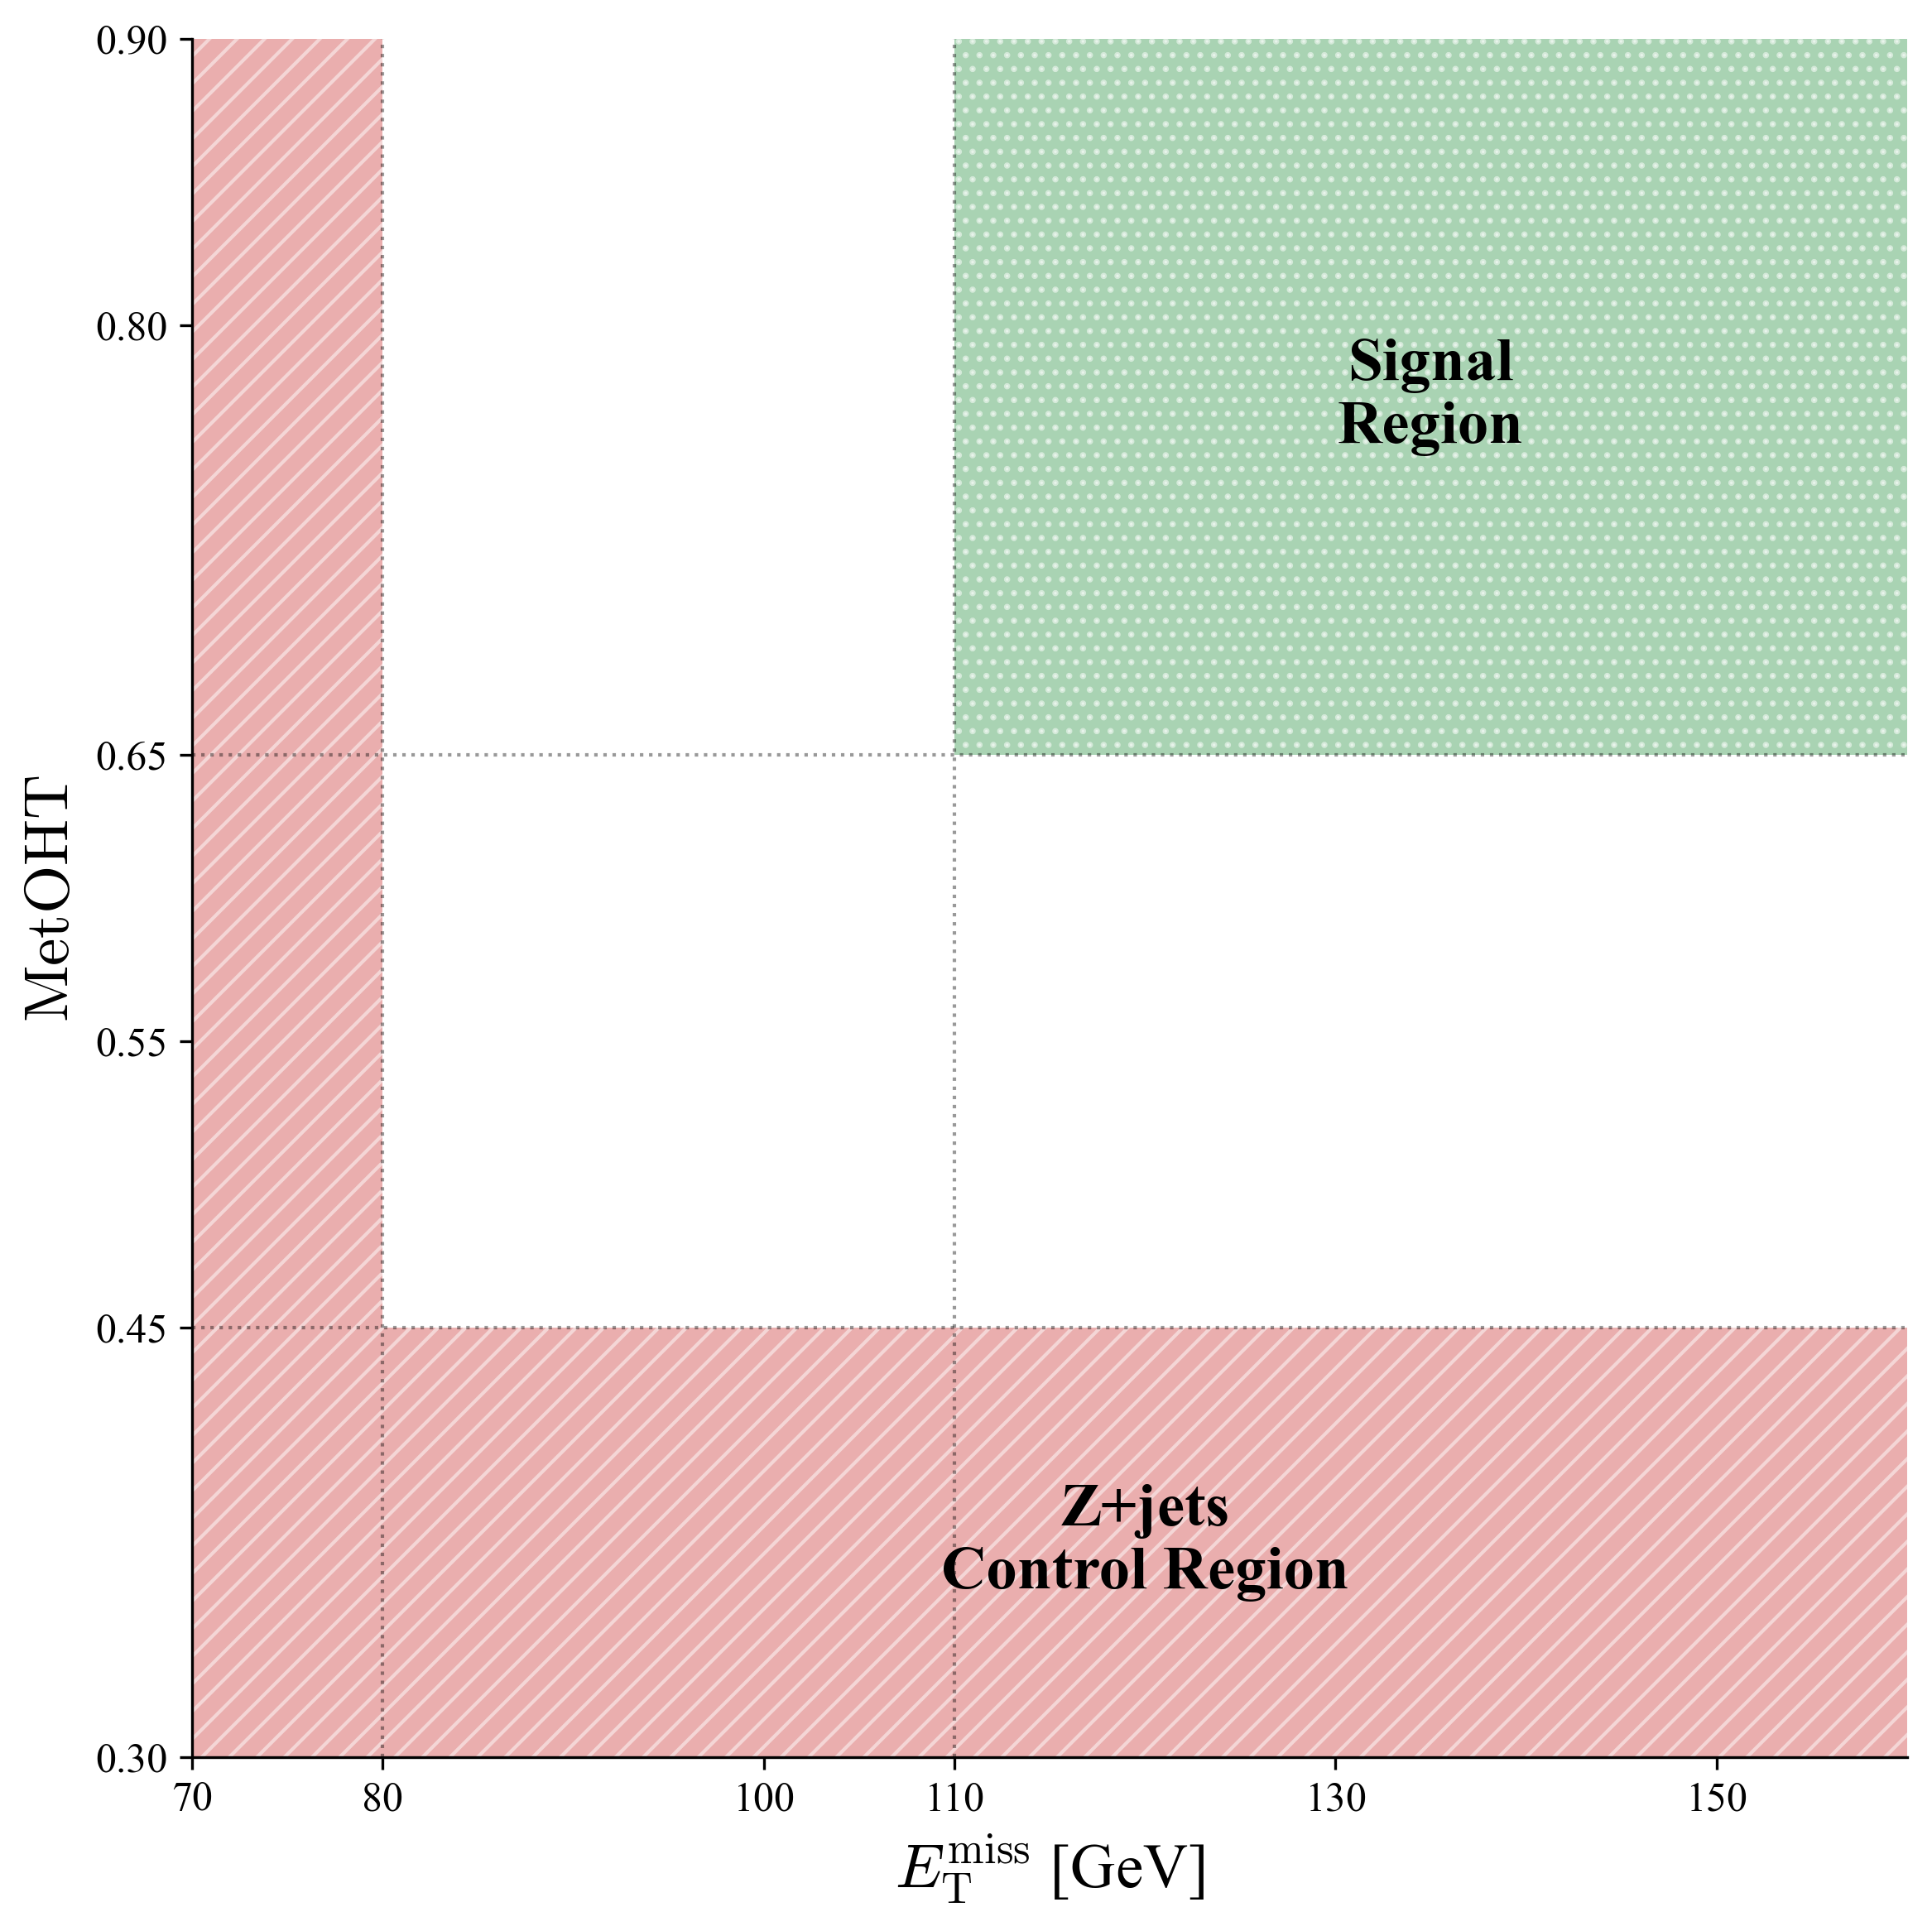
\includegraphics[width=0.6\textwidth]{figures/ch5-llvv/Zjets_Control_Region.png}
 \caption{Illustration of the inclusive phase-space in the ($E_{\text{T}}^{\text{miss}}$, $E_{\text{T}}^{\text{miss}}/H_{\text{T}}$) plane. The $\text{Z}$+jets Control Region is defined to be adjacent to the Signal Region to constrain the fake $E_{\text{T}}^{\text{miss}}$ tail while maintaining orthogonality.}
 \label{fig:Zjets_Control_Region}
\end{figure}

All other kinematic selections, such as the dilepton mass window ($80 < m_{\ell\ell} < 100~\text{GeV}$), lepton separation ($\Delta R_{\ell\ell} < 1.8$), and azimuthal separation ($\Delta \varphi(E_{\text{T}}^{\text{miss}}, \text{Z}) > 2.2$), are kept identical to the Signal Region to minimize extrapolation uncertainties. A summary of the cuts is provided in Table~\ref{table:Zjets_definition}.


\begin{table}[!htbp]
\centering
\begin{tabular}{|l|c|}
\hline
\textbf{Variable} & \textbf{Cut Value} \\ 
\hline 
Dilepton Mass & $80 < m_{\ell\ell} < 100~\text{GeV}$ \\
\hline 
\multirow{2}{*}{$E_{\text{T}}^{\text{miss}}$ / Significance} & ($70 < E_{\text{T}}^{\text{miss}} < 80~\text{GeV}$ \textbf{and} $E_{\text{T}}^{\text{miss}} / H_{\text{T}} > 0.3$) \\
& \textbf{OR} ($E_{\text{T}}^{\text{miss}} > 80~\text{GeV}$ \textbf{and} $0.3 < E_{\text{T}}^{\text{miss}} / H_{\text{T}} < 0.45$) \\
\hline 
Lepton separation & $\Delta R_{\ell\ell} < 1.8$ \\ 
\hline 
Azimuthal separation & $\Delta \varphi(E_{\text{T}}^{\text{miss}}, \text{Z}) > 2.2 $ \\
\hline 
Heavy Flavor & $b$-jet veto \\
\hline
\end{tabular}
\caption{Definition of the inclusive $\text{Z}$+jets Control Region. The region targets the phase space dominated by instrumental $E_{\text{T}}^{\text{miss}}$ while remaining orthogonal to the signal region.}
\label{table:Zjets_definition}
\end{table}

\subsubsection{Categorization by Jet Multiplicity}

Studies of the $\text{Z}$+jets modeling revealed significant shape differences between Data and Monte Carlo in key distributions used for unfolding. Since the fake $E_{\text{T}}^{\text{miss}}$ originates largely from jet mismeasurements, the kinematics of the event are strongly correlated with the number of hadronic jets. 

It was determined that a single global scaling factor was insufficient to correct the $\text{Z}$+jets prediction across the entire phase space. Therefore, the control region is split into three sub-regions based on jet multiplicity ($n_{\text{jets}}$):
\begin{itemize}
    \item $n_{\text{jets}} = 0$
    \item $n_{\text{jets}} = 1$
    \item $n_{\text{jets}} \ge 2$
\end{itemize}
Independent scaling factors are derived for each of these bins during the simultaneous fit. While a finer binning was investigated (separating $n_{\text{jets}}=2$ and $n_{\text{jets}} \ge 3$), results indicated that the scaling behavior was consistent for higher jet multiplicities, justifying the merged $\ge 2$ bin.

The pre-fit distributions of data and MC predictions in the $\text{Z}$+jets control regions (CRs) with three jet multiplicity categories are shown in Figure~\ref{fig:Zjet-CR} for the inclusive $\text{ZZ}$ analysis. The purity of $\text{Z}$+jets background events exceeds 95\% in these CRs. Although the observed data yields are higher than the MC predictions, they remain consistent within the associated uncertainties. In the final cross-section measurement, the normalization of the MC prediction will be determined through a simultaneous fit, which constrains the background contributions to the signal region.
For the VBS-like analysis, the $\text{Z}$+jets background is estimated using MC simulation due to the very limited statistics available in the $\text{ZZ}jj$ phase space. A conservative normalization uncertainty is assigned to this background in the fit to the $\text{ZZ}jj$ cross-section.

\begin{figure}[!htbp]
    \centering
    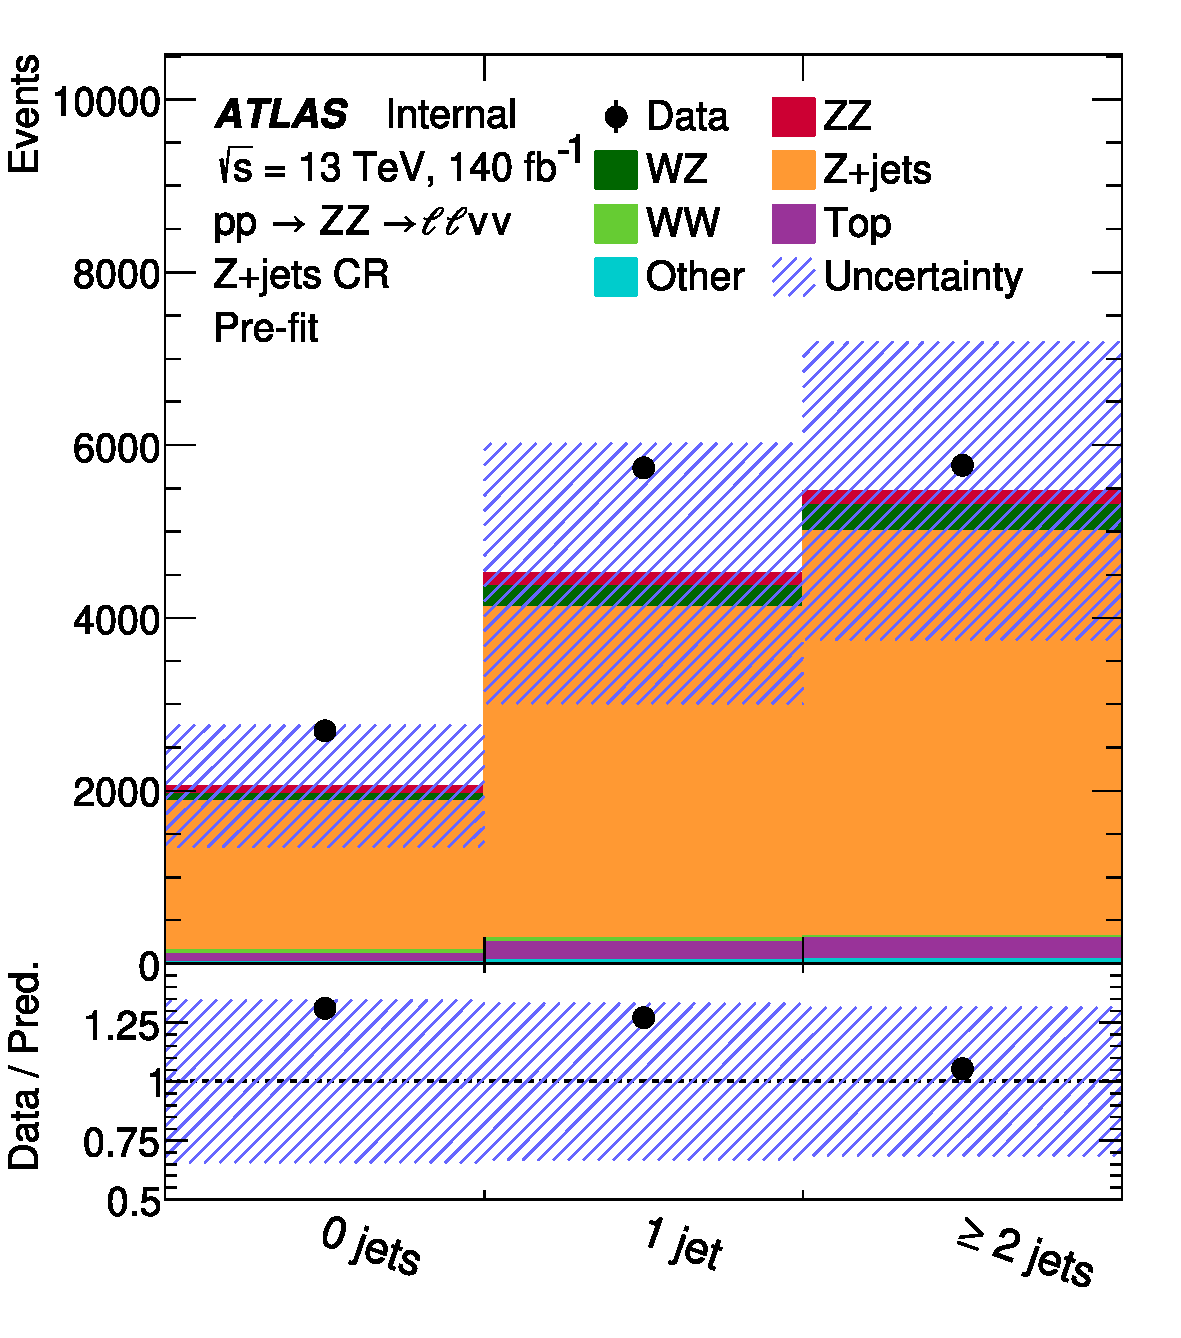
\includegraphics[width=0.5\linewidth]{figures/ch5-llvv/kin-distribution/Zj_VR_nJ-ZZ.pdf}
    \caption{Data and MC (pre-fit) comparison of the $\Delta\phi(\vec{E}_{\text{T}}^{\text{miss}}, \text{Z})$ in the $\text{Z}$+Jets CRs.}
    \label{fig:Zjet-CR}
\end{figure}

\subsubsection{Composition and Yields}

The pre-fit event yields for the inclusive $\text{Z}$+jets Control Region are detailed in Table~\ref{table:Zjets_unscaled}. 
\begin{table}[htbp]
\centering
\resizebox{\textwidth}{!}{%
\begin{tabular}{|l|c|c|c|}
\hline
\textbf{Process} & \textbf{$ee$ and $\mu\mu$} & \textbf{$ee$} & \textbf{$\mu\mu$} \\ \hline
\textbf{Data} & \textbf{14193.0 $\pm$ 119.13} & 6841.0 $\pm$ 82.71 & 7352.0 $\pm$ 85.74 \\ \hline
\hline
EWK & 11.62 $\pm$ 0.1 & 5.7 $\pm$ 0.07 & 5.92 $\pm$ 0.07 \\ \hline
QCD & 397.1 $\pm$ 5.98 & 183.28 $\pm$ 3.99 & 213.82 $\pm$ 4.45 \\ \hline
$\text{WZ}$ & 636.46 $\pm$ 7.49 & 301.33 $\pm$ 3.88 & 335.13 $\pm$ 6.41 \\ \hline
\textbf{$\text{Z}$+jets} & \textbf{10239.25 $\pm$ 176.43} & 4712.74 $\pm$ 120.55 & 5526.52 $\pm$ 128.83 \\ \hline
top, $t\bar{t}\text{V}$, $\text{W}t$ & 535.95 $\pm$ 5.94 & 262.62 $\pm$ 4.16 & 273.33 $\pm$ 4.24 \\ \hline
$\text{WW}$ & 113.04 $\pm$ 1.89 & 51.64 $\pm$ 1.28 & 61.4 $\pm$ 1.39 \\ \hline
Rare ($4\ell$, $\text{VVV}$, etc.) & 104.46 $\pm$ 4.38 & 54.65 $\pm$ 4.22 & 49.81 $\pm$ 1.19 \\ \hline
$\text{ZZ}$ & 408.72 $\pm$ 5.98 & 188.98 $\pm$ 3.99 & 219.74 $\pm$ 3.99 \\ \hline
\hline
\textbf{Total Bkg} & \textbf{11629.16 $\pm$ 176.76} & 5382.98 $\pm$ 120.77 & 6246.19 $\pm$ 129.07 \\ \hline
\hline
Data/MC & 1.18 $\pm$ 0.02 & 1.23 $\pm$ 0.03 & 1.14 $\pm$ 0.03 \\ \hline
$\frac{\text{Data-OtherBkg}}{\text{Zjets}}$ & 1.21 $\pm$ 0.03 & 1.27 $\pm$ 0.05 & 1.16 $\pm$ 0.05 \\ \hline
Signal/$\text{Z}$+jets (\%) & 3.99 $\pm$ 0 & 4.01 $\pm$ 0 & 3.98 $\pm$ 0 \\ \hline
\end{tabular}%
}
\caption{Pre-fit event yields in the inclusive $\text{Z}$+jets Control Region. The last row indicates the ratio of the Signal expectation to the dominant $\text{Z}$+jets background, confirming the region is background-enriched.}
\label{table:Zjets_unscaled}
\end{table}

The control region is dominated by $\text{Z}$+jets events, but shows a significant normalization discrepancy pre-fit, with Data exceeding the MC prediction by approximately 18\% in the inclusive selection. This reinforces the necessity of the data-driven scaling factors derived from this region. The signal contamination is controlled at the level of $\approx 4\%$.

%Validation of the simultaneous fit performance across these regions is detailed in Appendix~\ref{sec:TestScaled_3lCR}, while systematic uncertainties associated with the control region definitions and scaling factors are discussed in Section~\ref{sec:SystScaleFactorsCRvariations}.


\subsection{Minor Backgrounds}
\label{sec:bkg_minor}

Several background processes contribute to the signal region at a subleading level (typically $< 1\%$ of the total yield). Due to their small cross-sections or low acceptance in the analysis phase space, it is not feasible to define statistically significant dedicated control regions for these processes. Instead, their contributions are estimated purely from MC simulations normalized to their theoretical cross-sections.

These minor backgrounds include:

\begin{itemize}
    \item \textbf{$\text{ZZ} \to 4\ell$:} This process can enter the signal region if two leptons are lost (e.g., falling outside detector acceptance or failing identification). While physically similar to the signal, the requirement of large $E_{\text{T}}^{\text{miss}}$ strongly suppresses this contribution.
    
    \item \textbf{Triboson Production ($\text{VVV}$):} Processes such as $\text{WWW}$, $\text{WWZ}$, and $\text{WZZ}$ have very small production cross-sections but can produce high lepton multiplicities and missing energy.
    
    \item \textbf{$t\bar{t}\text{V}$ ($t\bar{t}\text{Z}$, $t\bar{t}\text{W}$):} Associated production of top pairs with a boson. These events are largely rejected by the $b$-jet veto applied in the signal region.
    
    \item \textbf{$\text{W}$ + jets:} Events where a $\text{W}$ boson decays leptonically and a jet is misidentified as a second lepton. Strict lepton identification and isolation criteria employed in this analysis reduce this background to a negligible level.
\end{itemize}

Since these backgrounds are not constrained by data in the simultaneous fit, conservative systematic uncertainties are assigned to their theoretical cross-sections (typically on the order of $20\%$ to $30\%$) to account for potential modeling discrepancies.

\subsection{Summary of the Data and MC Yields from SRs and CRs}
\label{sec:summary-table}

Data and pre-fit MC yields for the inclusive $\text{ZZ}$ phase space are presented in Table~\ref{tab:prefitYieldsInclu}. The predicted signal-to-background ratio in the signal region (SR) is approximately 1.5. The targeted background control regions exhibit high purity: for example, the top-quark purity in the non-resonant CR with a $b$-jet requirement is close to 100\%, while the $\text{WZ}$ purity in the $\text{WZ}$ CR exceeds 90\%.


\begin{table}[htbp]
    \centering
    \renewcommand{\arraystretch}{1.2}
    \resizebox{\textwidth}{!}{%
    \begin{tabular}{lccccccc}
       \hline
\textbf{Process} & \textbf{SR} & \textbf{$\text{WZ}$ CR} & \textbf{$\text{WW}$ CR} & \textbf{Top CR}
& \textbf{$\text{Z}$+0j CR} & \textbf{$\text{Z}$+1j CR} & \textbf{$\text{Z}+\ge 2\text{j}$ CR} \\
       \hline
        $\text{ZZ}$ signal     & 1650 (36)    & 2.6 (0.7)    & 0.58 (0.11)  & 0.005 (0.011) & 100 (12)     & 150 (20)      & 160 (34)      \\
        \hline \hline
        \textbf{Background} &  & & & & & & \\
        \hline
        $\text{WZ}$            & 740 (43)     & 2100 (140)   & 22 (2)       & 0.9 (0.3)    & 80 (12)      & 250 (28)      & 310 (60)      \\
        $\text{Z}$+0j          & 80 (34)      & 40 (17)      & 0.6 (1.0)    & 0            & 1700 (670)   & 0             & 0             \\
        $\text{Z}$+1j          & 80 (40)      & 40 (14)      & 2.2 (0.7)    & 0.12 (0.08)  & 0            & 3800 (1460)   & 0             \\
        $\text{Z}+\ge 2\text{j}$ & 13 (7)       & 20 (12)      & 0.4 (0.6)    & 0.15 (0.16)  & 0            & 0             & 4700 (1700)   \\
        $\text{WW}$            & 36.2 (1.9)   & 0.65 (0.12)  & 672 (41)     & 13.9 (1.6)   & 48 (6)       & 46 (5)        & 18.5 (1.9)    \\
        Top                    & 114 (20)     & 57 (8)       & 1850 (290)   & 5700 (710)   & 92 (25)      & 200 (39)      & 250 (43)      \\
        Other                  & 48 (4)       & 91 (7)       & 46 (13)      & 3.4 (1.3)    & 12 (3)       & 44 (10)       & 48 (10)       \\
       \hline
        Total prediction       & 2760 (120)   & 2340 (150)   & 2590 (310)   & 5720 (710)   & 2050 (700)   & 4510 (1500)   & 5470 (1700)   \\
        \hline \hline
        \textbf{Data}          & \textbf{2917} & \textbf{2409} & \textbf{2903} & \textbf{5736} & \textbf{2691} & \textbf{5733} & \textbf{5769} \\
       \hline
    \end{tabular}}
    \caption{Data and pre-fit MC yields for the inclusive $\text{ZZ}$ phase-space. The ``Other'' category includes events from the processes $\text{ZZ} \to 4\ell, 2\ell 2q$, $\text{VVV}~(\text{V}=\text{W,Z})$, $\text{W}j$, $\text{Z} \to \tau\tau$, and $\text{WH}$. The selected number of data events in the SR and the CRs is also provided. The numbers shown in the parentheses are the MC uncertainties.}
    \label{tab:prefitYieldsInclu}    
\end{table}

Data and pre-fit MC yields for the VBS-like $\text{ZZ}jj$ phase space are presented in Table~\ref{tab:prefitYieldsZZjj}. The predicted signal-to-background ratio in the signal region (SR) is approximately 1.45. The overall Top+$\text{WW}$ purity in the non-resonant CR is 97\%, while the $\text{WZ}$ purity in the $\text{WZ}$ CR is 88\%.


\begin{table}[htbp]
    \centering
    \small
    \renewcommand{\arraystretch}{1.2}
    \begin{tabular}{lccc}
       \hline
\textbf{Process} & \textbf{SR} & \textbf{$\text{WZ}$ CR} & \textbf{$\text{WW}$ and Top CR} \\
       \hline
        $\text{ZZ}$ signal     & 108 (12)   & 1.0 (0.3)  & 0.006 (0.004) \\
        \hline
        \hline
        \textbf{Background} &  & &  \\
        \hline        
        $\text{WZ}$            & 62 (12)    & 280 (60)   & 4.8 (1.0)     \\
        $\text{Z}$+jets        & 2.4 (1.2)  & 15 (8)     & 0.4 (0.2)     \\
        $\text{WW}$ and Top    & 7.2 (1.5)  & 8.2 (1.8)  & 620 (90)      \\
        Other                  & 3.0 (0.7)  & 12 (3)     & 12 (14)       \\
       \hline
        Total prediction       & 183 (21)   & 320 (60)   & 640 (100)     \\
        \hline \hline
       \textbf{Data}           & \textbf{184} & \textbf{317} & \textbf{678} \\
       \hline
    \end{tabular}
    \caption{Data and pre-fit MC yields for the $\text{ZZ}jj$ phase-space. The ``Other'' category includes events from the processes $\text{ZZ} \to 4\ell, 2\ell 2q$, $\text{VVV}~(\text{V}=\text{W,Z})$, $\text{W}j$, $\text{Z} \to \tau\tau$, and $\text{WH}$ production. The selected number of data events in the SR and the CRs is also provided in the table. The numbers shown in the parentheses are the MC uncertainties.}
    \label{tab:prefitYieldsZZjj}
\end{table}


